%%%%%%%%%%%%%%%%%%%%%%%%%%%%%%%% 
\section{The Cold Electronics (CE)} 
\label{sec:detectors-fd-ref-ce}

The TPC read-out electronics are mounted on the APA front-end
(Figure~\ref{fig:elec_CMBonAPA}) in LAr.  These electronics are
therefore referred to as the ``Cold Electronics'' (CE) subsystem.  The
scope of the CE subsystem includes the design, procurement,
fabrication, testing, delivery and installation of the CE, the
principal components of which are:
\begin{itemize}
\item front-end electronics cards installed on the APAs;
\item signal feedthroughs mounted on the cryostat;
\item power supplies and cabling.
\end{itemize}
The most significant requirements for the CE are to:
\begin{itemize}	
\item minimize channel capacitance and noise
\item minimize dissipated power per channel in the LAr
\item read out the TPCs and transmit their data to the DAQ
\item record the channel waveforms continuously without dead time
\item provide sufficient precision and range to satisfy the Key Physics Parameters
\item operate for the life of the facility without significant loss of function
\item use only materials that are compatible with high-purity liquid argon and minimal natural radioactivity
\end{itemize}
\begin{cdrfigure}[The front-end electronics as mounted on an APA]{elec_CMBonAPA}
 {The front-end electronics, shown in the red circle, as mounted on an APA.}
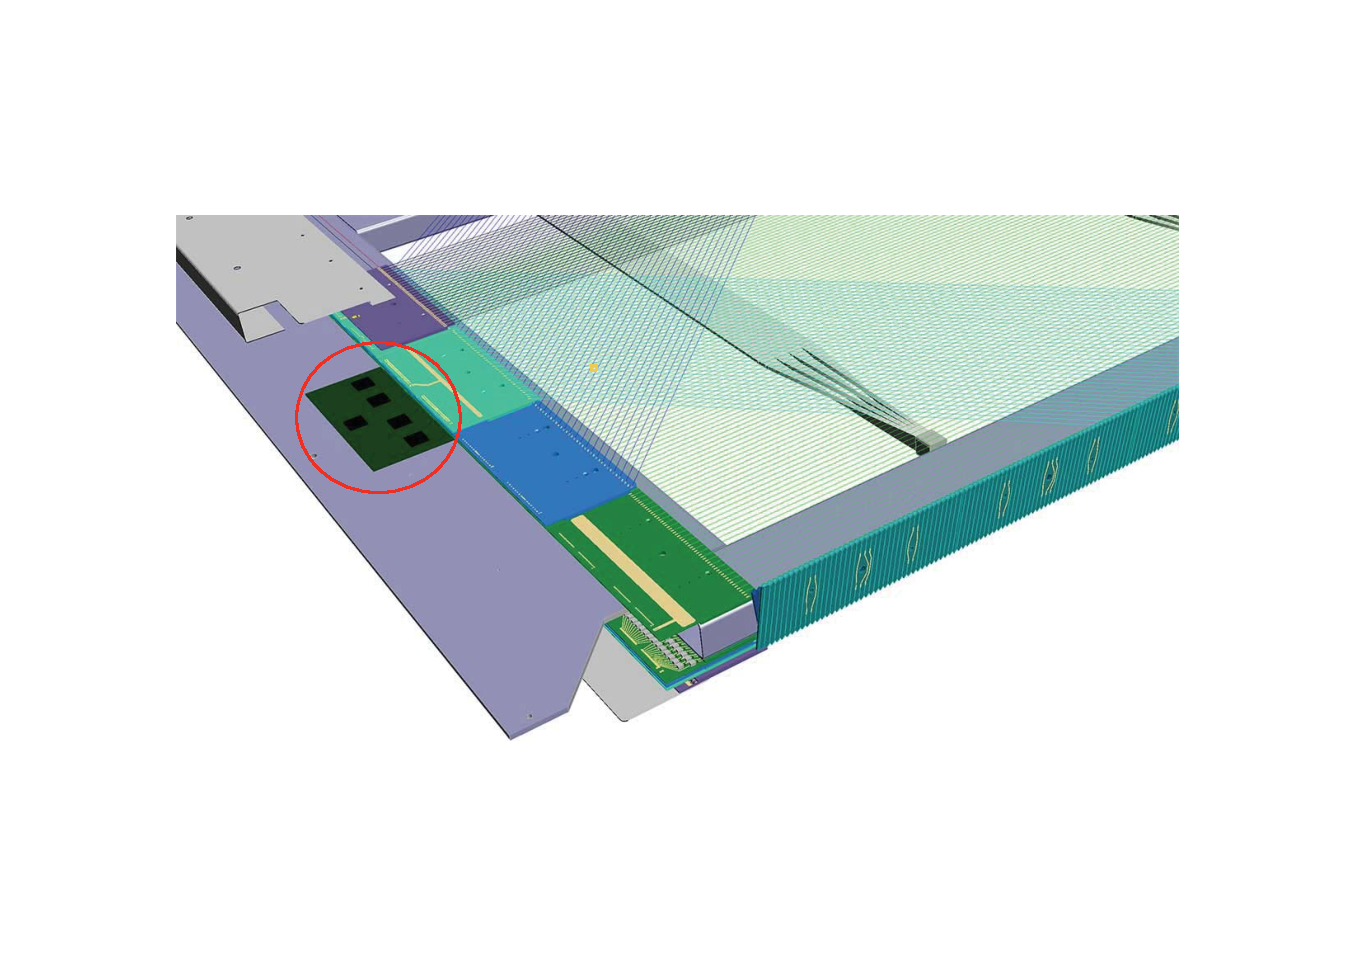
\includegraphics[width=0.70\linewidth]{elec_CMBonAPA_1.pdf}
\end{cdrfigure}

The CE are implemented as ASIC chips using CMOS technology, which
performs well at LAr temperatures~\cite{ThornEtAl:CELAr}, and provides
amplification, shaping, digitization, buffering and multiplexing (MUX)
of the signals.  The CE architecture is manifested in the Front End
Mother Board (FEMB), a 128-channel board which uses eight 16-channel
Front End (FE) ASICs and eight 16-channel ADC ASICs
(Figure~\ref{fig:elect_schem}).  The FE ASIC provides amplification
and pulse shaping, while the ADC ASIC comprises a 12-bit digitizer and
an 8:1 MUX stage with two pairs of serial readout lines in parallel.
A Cold Digital Data (COLDATA) ASIC chip
(Fig.~\ref{fig:elec_COLDATAfig}) mounted on each FEMB provides an
additional MUX of 4:1 and is capable of driving the data at 1~Gb/s
through 30~m of copper cable to the feedthrough and on to the DAQ.
Tables~\ref{tab:DeviceCounts} and \ref{tab:KeyParameters} list the CE
device counts and key parameters.
%\vskip -10pt % This prevents the last table from appearing in the PD section by pulling the figure up, which is easily accomodated.
\begin{cdrfigure}[The Cold Electronics Architecture]{elect_schem}
{
  The CE Architecture. The basic unit is the 128-channel FEMB. FEASIC: Front End ASIC.
  PA: Pre-amplifier.  $\int$: Shaper.  MUX: Multiplexer.  Drv: Driver.
}
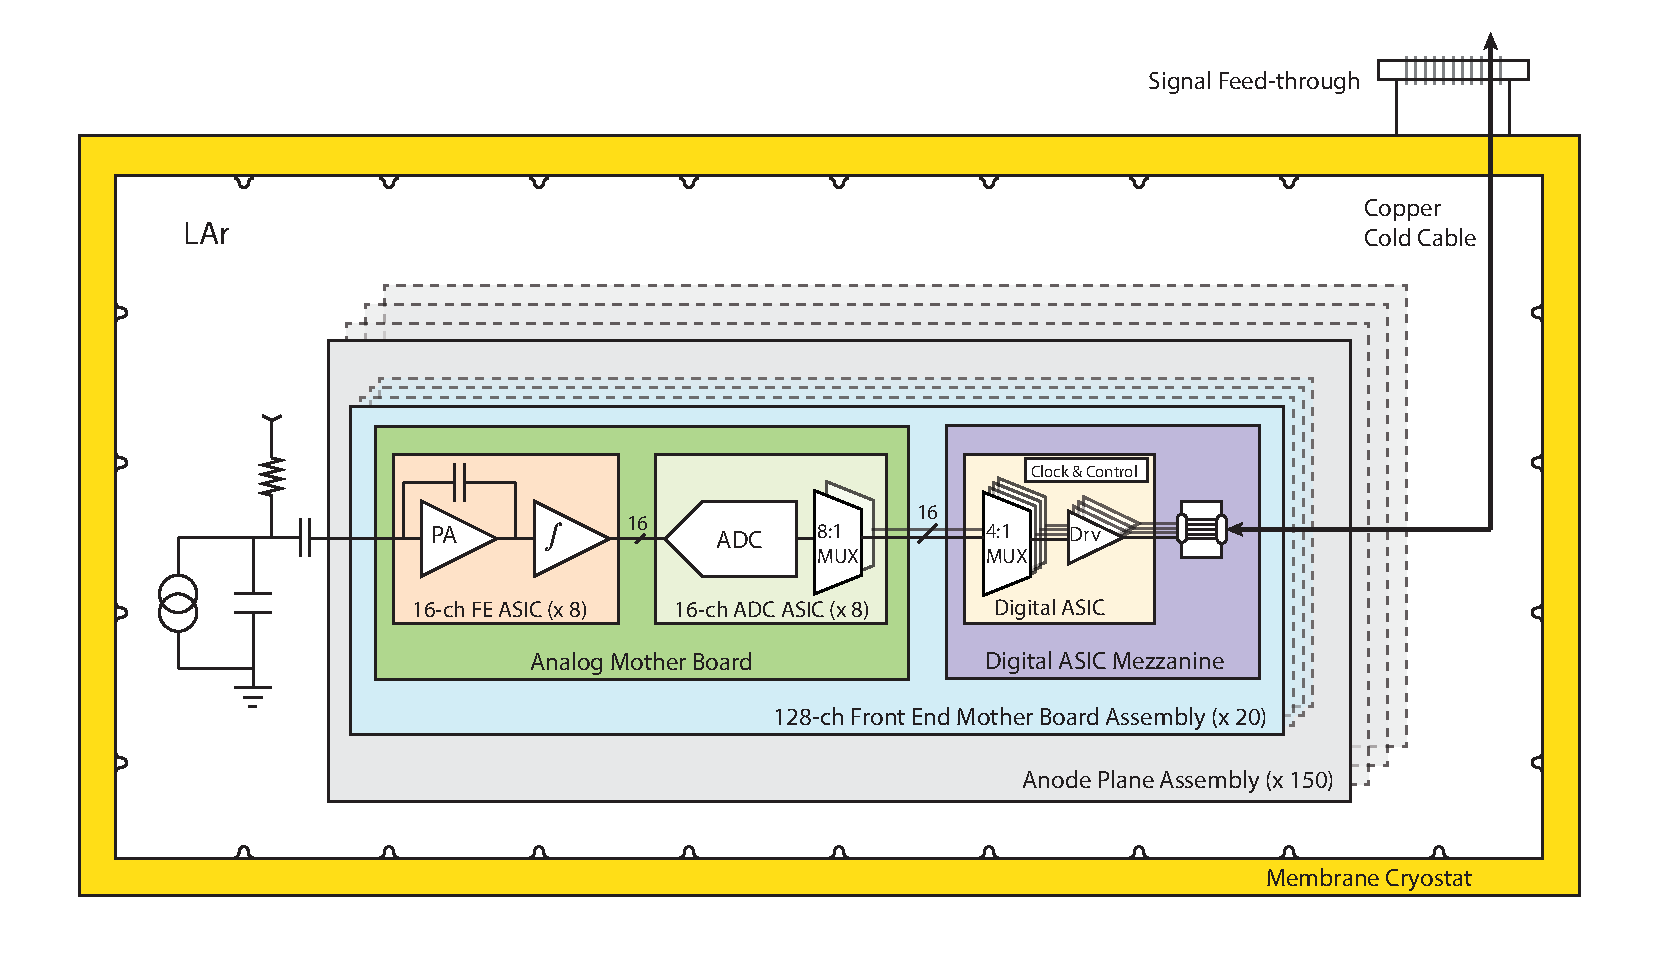
\includegraphics[width=0.90\linewidth]{elect_schem.pdf}
\end{cdrfigure}
\begin{cdrfigure}[Functional Block Diagram of the COLDATA ASIC]{elec_COLDATAfig}
{Functional Block Diagram of the COLDATA ASIC. PLL: Phase Locked Loop.  VCXO: Voltage-Controlled Crystal Oscillator}
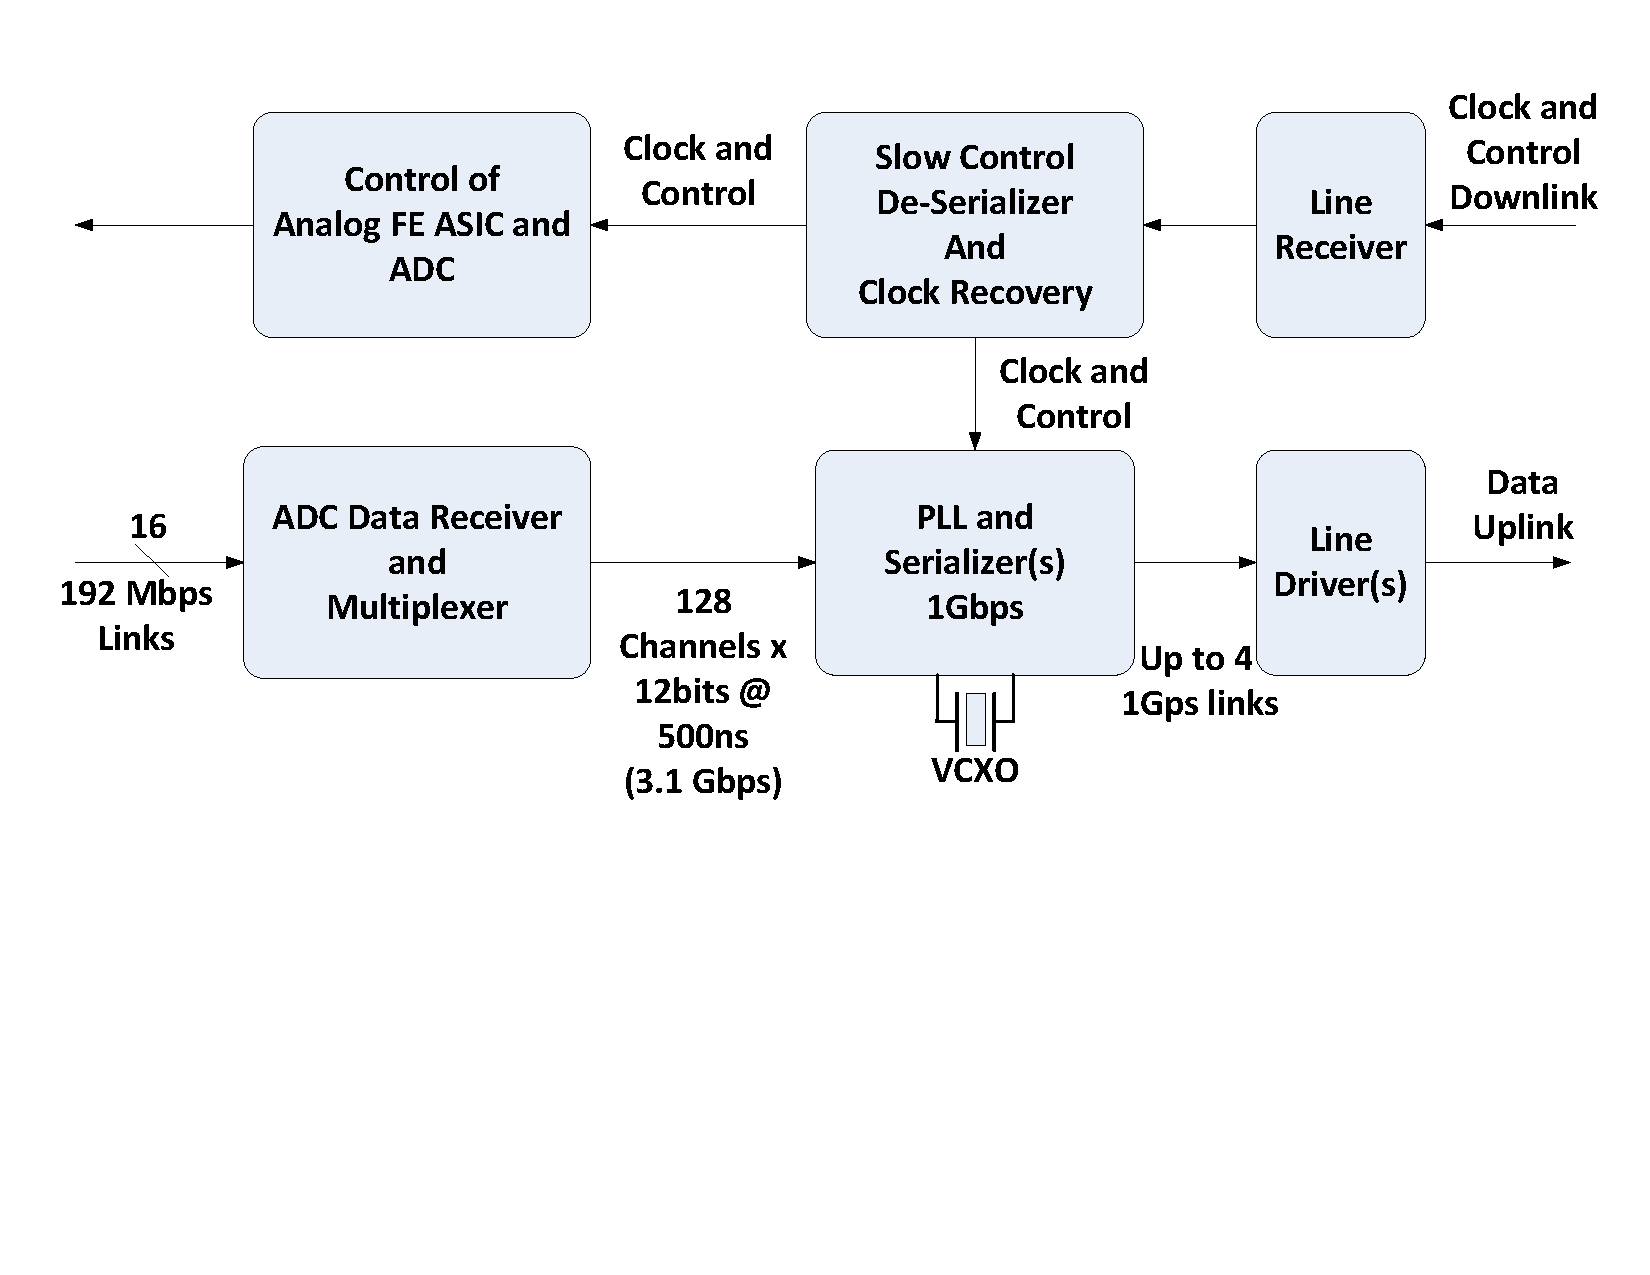
\includegraphics[width=0.80\linewidth]{elec_COLDATAfig.pdf}
\end{cdrfigure}

An important aspect of CMOS technology is that the lifetime at
cryogenic temperatures is well understood and can be well controlled,
{\em provided that close control is maintained over the implementation
  details}.  This precludes the use of commercial devices, which are
not intended for use in LAr, and which are produced by proprietary
processes over which DUNE has no control.
% This requirement of close control cannot be satisfied by any commercial device,
% where the manufacturing process is subject to change.
% Strict requirements in industry to deliver a device with equivalent performance and lifetime,
% despite a change in the proprietary manufacturing process or technology,
% only applies to a range of temperatures which does {\em not} include LAr temperatures.
% Performance and accelerated-lifetime testing of commercial devices will not protect against 
% a substantially different performance or shorter lifetime in the cold following a manufacturing process change
% over which we have no control, nor necessarily any knowledge.
% It is because of this serious concern that we are undertaking the development and fabrication of our own devices, 
% so that tight control of the process can be maintained.
It is worth noting that the FEMB, together with the FE and ADC ASIC
chips, has already been prototyped and tested using a commercial FPGA
to perform the role of the COLDATA ASIC, which is currently under
development.  The 1-Gb/s data rate can be achieved with copper links
and without zero suppression or data compression.
% is not high enough to require the use of optical fibers in the cold,
% nor is there a need for zero suppression or data compression.
This greatly reduces the complexity of the COLDATA ASIC, with a
corresponding decrease in overall risk, including risk of
failure-to-implement (within a fixed schedule and budget).  The
COLDATA work is especially challenging, with final production not
scheduled to begin until late 2019.  Alternative approaches are
currently under study.

\begin{cdrtable}[Cold Electronics Device Counts]{l|r|r|r}{DeviceCounts}{CE Device Counts}
 Parameter           & per FEMB& per APA& per 10~kt Detector\\ \toprowrule
 Channels            & 128    & 2560   & 384,000           \\ \colhline
 FE \& ADC ASIC Chips&   8    &  160   &  24,000           \\ \colhline
 COLDATA ASIC Chips  &   1    &   20   &   3,000           \\ \colhline
 FEMB                &   1    &   20   &   3,000           \\ \colhline
 Signals-Out         &   4    &   80   &  12,000           \\ \colhline
 APA                 & ---    &    1   &     150           \\
\end{cdrtable}
\begin{cdrtable}[Cold Electronics Key parameters]{l|l}{KeyParameters}{CE Key parameters}
 Parameter                &  Value                               \\ \toprowrule
 Signal-to-Noise (in LAr) &  9:1 for 1~$\mu$s peaking time       \\ \colhline
 MUX Level                &  32                                  \\ \colhline
 Sampling Frequency       &  2~MHz                               \\ \colhline
 ADC Resolution           &  12~bits                             \\ \colhline
 FE Peaking Time          &  0.5, 1, 2, 3~$\mu$s (selectable)    \\ \colhline
 FE Gain                  &  4.7, 7.8, 14, 25~mV/fC (selectable) \\ \colhline
 Calibration Precision    &  1\%                                 \\ \colhline
 Power dissipation        &  11~mW/channel                       \\
\end{cdrtable}
